\documentclass{article}

% Esto es para poder escribir acentos directamente:
\usepackage[latin1]{inputenc}
% Esto es para que el LaTeX sepa que el texto est� en espa�ol:
\usepackage[spanish]{babel}

\usepackage{graphicx}

%Ruta absoluta en formato tipo Unix (Linux, OsX, Windows)
\graphicspath{ {C:\Users\User\Desktop\Estructura-de-Datos} }

%--------------------------------------------------------------------------

\title{Ejemplo  C++ Punteros}
\author{Michael Daniel Murillo L�pez\\
\small ID:534830\\
\small Estructura de Datos\\
\small Corporaci�n Universitaria Minuto de Dios    \\
\small  Uniminuto\\
\small \\
\small \\
\small \\
\small Bogota D,C\\
}

\begin{document}
\maketitle

\section{C�digo:}

\LARGE El siguiente documento nos presentar� el paso a paso de un ejemplo que se realizo en c++ donde manejamos los punteros en dos tipos que son:

* Ir a la direcci�n de memoria 


* La posici�n. 


Explicaremos cada l�nea de c�digo en un peque�o resumen tambi�n mostrando el pantallazo de nuestro programa para que quien lo lea nos entienda mejor.

\begin{figure}
  \centering
   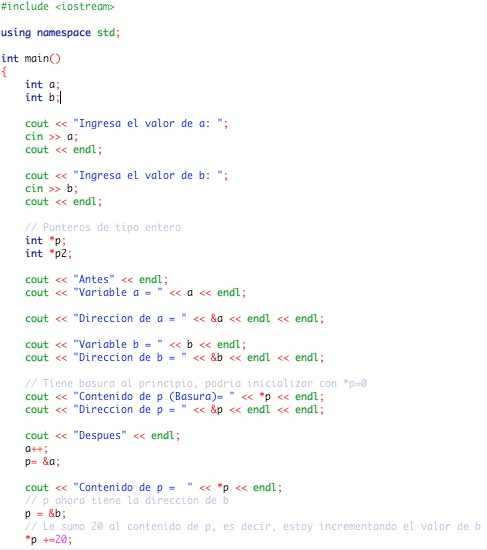
\includegraphics[width=1\textwidth]{captura}
   
En primer lugar creamos la clase main() y declaramos dos variables a y b de tipo entero (int) y luego cargamos cada una pidiendo que el usuario ingrese el valor de las mismas, luego de esto creamos los punteros para las variables nombradas anteriormente e imprimimos el valor que tiene cargado cada variable y su direcci�n en memoria, as� mismo tambi�n nos trae el contenido que tiene la variable de ese puntero. Luego a la variable 'a' le sumamos 1 e imprimimos el puntero 'p' con su direcci�n en memoria. Luego de esto a 'p' se le da la direcci�n de 'b' y se le suma 20.
   
  \caption{Captura 1}
  \label{fig:ejemplo}
\end{figure}


\begin{figure}
  \centering
   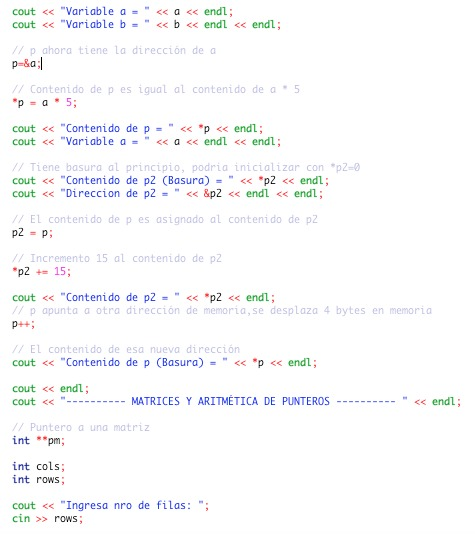
\includegraphics[width=1\textwidth]{captura2}
   
Aca imprimimos la variable 'a' y 'b' con los cambios y sumatorias hechos anteriormente, a 'p' se le da la direcci�n de memoria de la variable 'a' para luego a esta misma multiplicarla por 5, luego imprimimos la direcci�n del puntero 'p' y el contenido de ese mismo puntero. El segundo puntero 'p2' lo igualamos al primer puntero 'p' y le incrementamos 15 para luego imprimir el contenido de 'p2'. Luego de esto a 'p' se le suma 1 y se imprime su direcci�n de memoria y finalizamos estas matrices. Inmediatamente comenzamos con las Matrices y Aritm�tica de punteros, donde declaramos un puntero a otro puntero de una matriz 'pm', tambi�n creamos dos variables 'cols' y 'rows' como enteros (int) y le pedimos al usuario el n�mero de filas que desea.
   
  \caption{Captura 2}
  \label{fig:ejemplo}
\end{figure}

\begin{figure}
  \centering
   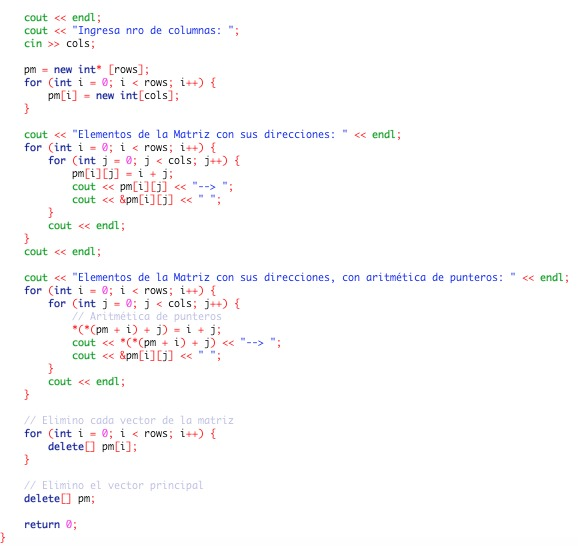
\includegraphics[width=1\textwidth]{captura3}
  
En esta empezamos pidiendo al usuario el n�mero de columnas que desea. Luego de esto igualamos la matriz 'pm' al puntero de 'rows' para luego iterar por medio de un ciclo for entre filas y columnas de la matriz 'pm'. Luego de esto imprimimos a trav�s de un ciclo for anidado los elementos de la matriz con sus respectivos contenidos de cada posici�n de la matriz. Luego de esto y tambi�n gracias a un ciclo for anidado imprimimos los elementos de la matriz con sus direcciones pero con la aritm�tica de punteros y al final eliminamos cada vector de la matriz con el vector principal de 'pm' y retornamos 0.
 \caption{Captura 3}
  \label{fig:ejemplo}
\end{figure}
  


\end{document}